\subsubsection{{Выбор архитектуры системы}}
\addcontentsline{toc}{subsubsection}

Общий вид системы для автоматического проектирования генеральных планов площадных объектов можно представить в виде
двух независимых друг от друга частей: бизнес-части и расчётной.
Эти части системы схематично изображены на диаграмме ниже(см. рисунок \ \ref{pic:architecture__system-diagram}).

\begin{figure}[H]
	\hspace*{-2.5 cm}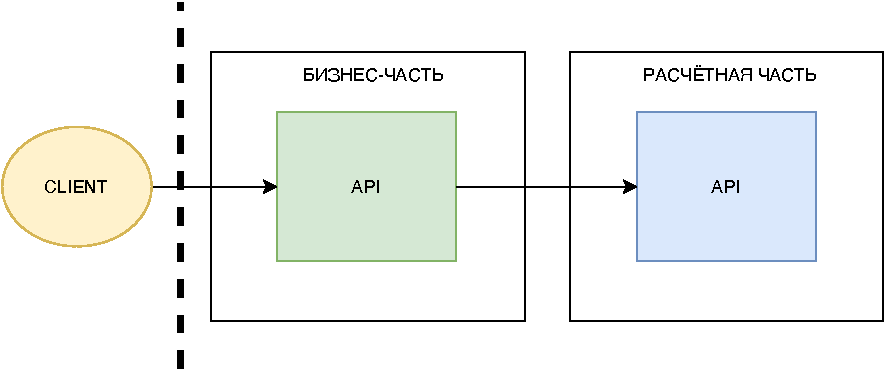
\includegraphics[width=0.8\textwidth, left]{architecture/pictures/common/system}
	\caption{Общий вид системы}
	\label{pic:architecture__system-diagram}
\end{figure}
\vskip 5 mm

Бизнес-часть приложения используется для отображения полученных результатов внешним экспертам со стороны заказчика.
Именно в этой части определены все правила и те объекты, которые используются в экспертной оценке.
В расчётной части системы используются объекты внутренней модели данных.
Эти внутренние объекты уже не могут быть интерпретированы внешними экспертами.

Также стоит отметить, что внутренняя модель данных подвержена сильным изменениям в процессе исследований.
Новые алгоритмы решения задачи могут давать куда более качественный результат, но только с учетом того, что
будут использованы дополнительные структуры данных. В то время как внешняя модель данных относительно стабильна
и представлена объектами целиком и полностью понятными внешним экспертам.

Целью данной работы является проектирование и реализация только расчётной части системы, поэтому на всех остальных
диаграммах представленных в работе рассматривается именно эта часть.

Для удовлетворения описанных в предыдущей главе требований предлагается архитектура системы,
использующая микросервисный подход. Данный подход позволяет разбить систему на отдельные блоки,
каждый из которых будет выполнять только свою задачу и не зависеть от функционала других блоков.
Независимость каждого из сервисов существенно упростит процесс разработки и отладки в силу изолированности
каждой задачи. Помимо этого каждый сервис может быть развернут отдельно от остальных, в зависимости
от требований распределения нагрузки. Микросервисный подход к разработке позволит разрабатывать
автономные и слабосвязанные друг с другом сервисы.

Для решения поставленной задачи предлагается следующая архитектура расчётного
модуля(см. рисунок \ \ref{pic:architecture__common-component}).

\begin{figure}[H]
	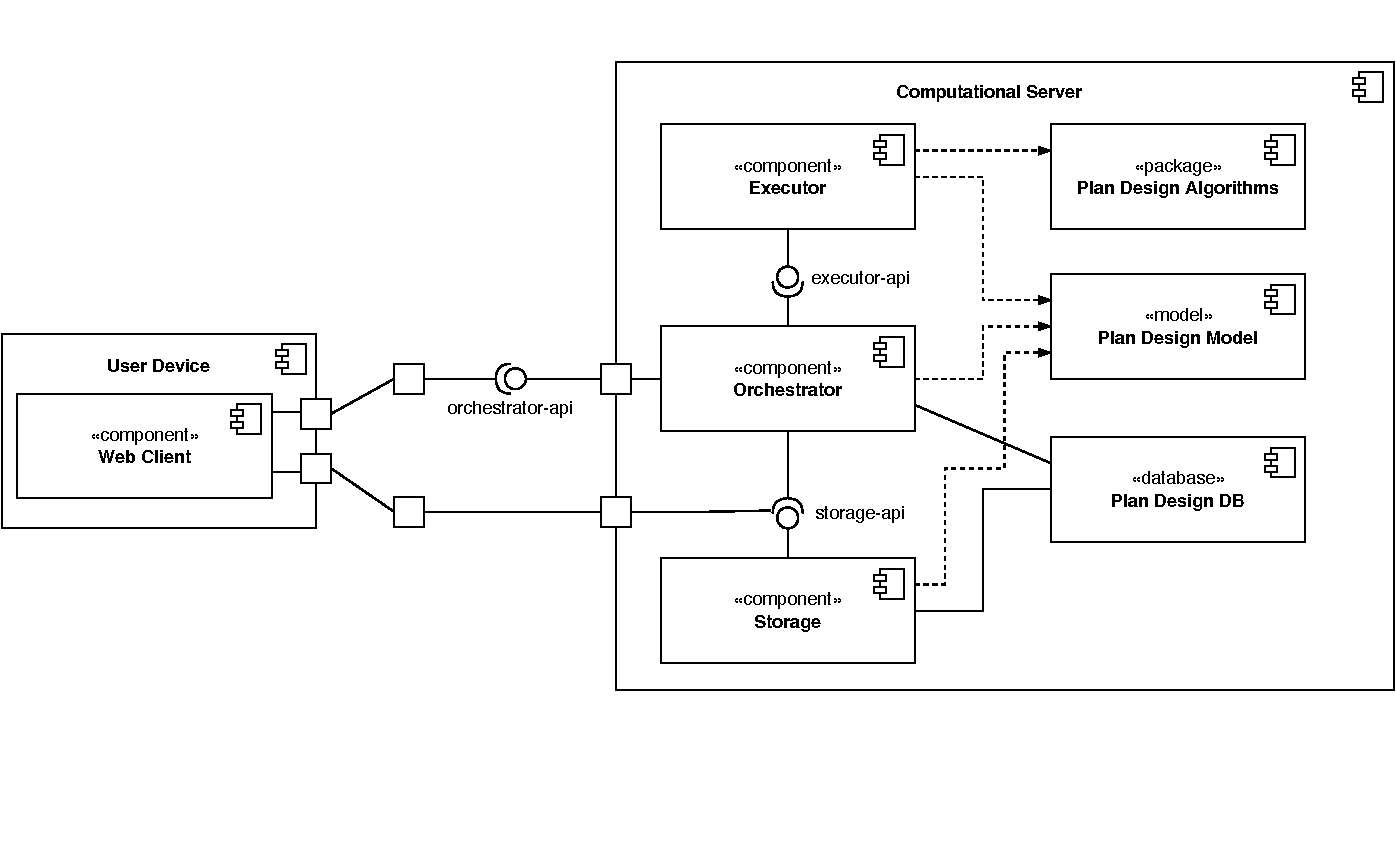
\includegraphics[width=\textwidth, left]{architecture/pictures/common/component}
	\caption{Верхнеуровневая диаграмма компонентов}
	\label{pic:architecture__common-component}
\end{figure}
\vskip 5 mm

Схема развертывания компонентов, указанных выше, изображена на диаграмме
развёртывания(см. рисунок \ \ref{pic:architecture__common-deployment}).
\begin{figure}[H]
	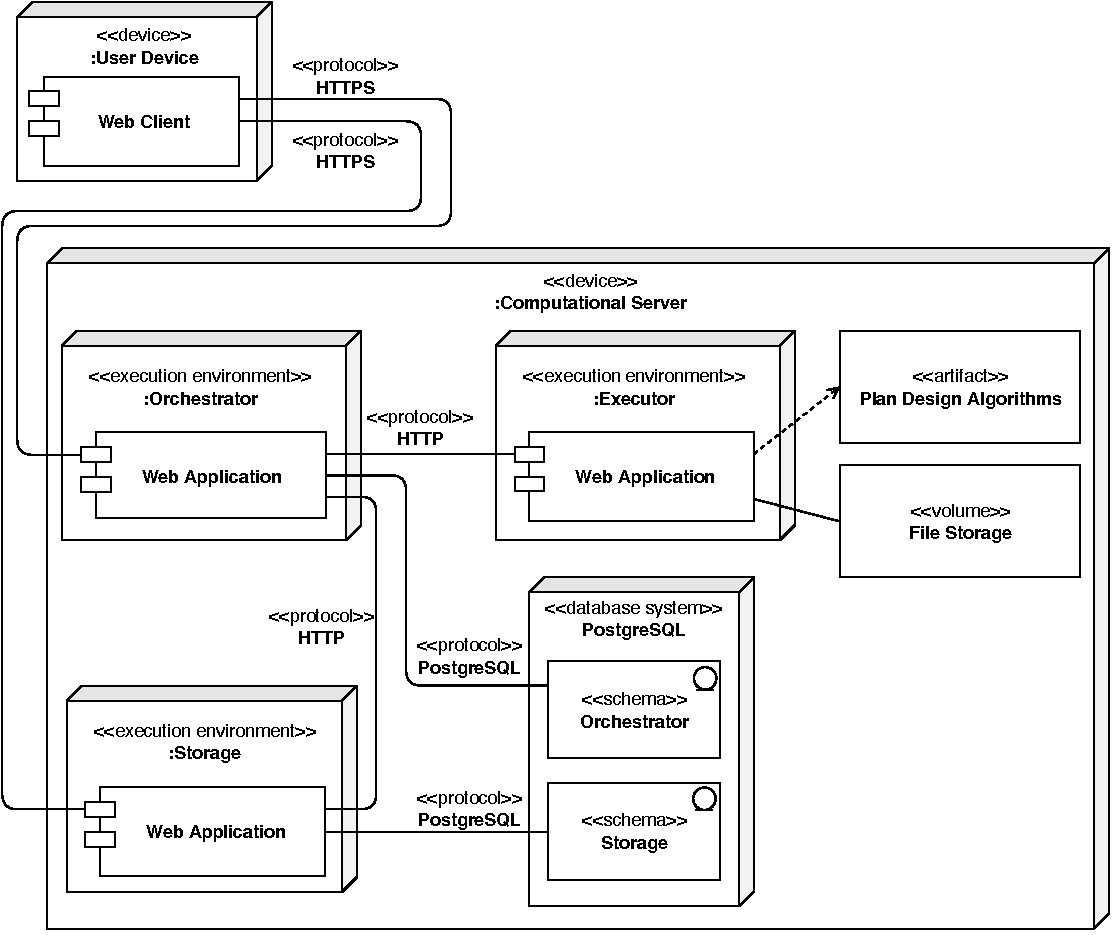
\includegraphics[width=\textwidth, left]{architecture/pictures/common/deployment}
	\caption{Диаграмма развёртывания}
	\label{pic:architecture__common-deployment}
\end{figure}
\vskip 5 mm

\noindent Объекты представленные на диаграмме компонентов:
\begin{itemize}
	\item \textit{Computational Server} -- сервер для запуска расчётных задач.
	\item \textit{Plan Design Algorithms} -- математическая библиотека, содержащая алгоритмы
	для построения генеральных планов.
	\item \textit{Plan Design Model} -- расчётная модель данных.
	\item \textit{Executor} -- сервис, отвечающий за запуск методов математической библиотеки.
	\item \textit{Storage} -- сервис, отвечающий за чтение/запись расчётной модели данных.
	\item \textit{Orchestrator} -- сервис, контролирующий выполнение расчётных задач.
	\item \textit{File Storage} -- файловое хранилище.
	\item \textit{Plan Design DB} -- база данных.
\end{itemize}

Самой ресурсоёмкой частью приложения является запуск математических методов.
Сервис \textit{Executor}, отвечающий за это, отвязан от использования других компонент системы
и может работать полностью изолированно.
Поэтому, в случае необходимости, возможно оперативное развертывание нескольких экземпляров данного сервиса
на других вычислительных узлах.

Так как проект является исследовательским, то основными пользователями является немногочисленная команда проекта.
Поэтому использование дополнительных архитектурных компонент,
таких как балансировщики нагрузки и системы автоматического развертывания новых экземпляров приложения
здесь просто не требуется.

Основной причиной применения микросервисного подхода в данном случае является изолированность задач с целью
упрощения проведения исследований.
В монолитном приложении из-за высокой связности между компонентами спустя время становится крайне сложно добавление
нового функционала. В исследовательских проектах в силу неопределенных требований это очень важное ограничение,
которое в какой-то момент просто может не позволить дальше продолжать
научные изыскания без переработки архитектуры проекта.
